\chapter{Trees and spanning trees}
\section*{A network without redundancy}
A connected network with no cycles has exactly one simple route between any two vertices. Such a network is called a tree. Trees arise in family histories, file systems, communication backbones and efficient ways of linking locations.

\begin{definition}
A \emph{tree} is a connected graph with no cycles. A \emph{forest} is a graph with no cycles; each of its connected components is a tree. A \emph{spanning tree} of a graph is a subgraph that is a tree and contains every vertex of the original graph. A \emph{leaf} (or \emph{pendant vertex}) is a vertex of degree 1.
\end{definition}

\begin{figure}[htbp]
\centering
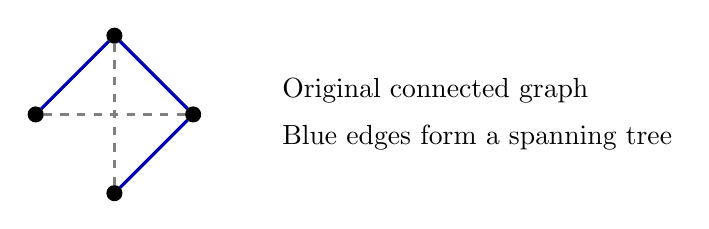
\begin{tikzpicture}[thick,vertex/.style={circle,draw=black,fill=black,inner sep=0pt,minimum size=5pt}]
\node[vertex] (a) at (0,0) {}; \node[vertex] (b) at (1,1) {}; \node[vertex] (c) at (2,0) {}; \node[vertex] (d) at (1,-1) {};
\draw[gray,dashed] (a)--(c) (b)--(d);
\draw[blue!70!black,line width=1.2pt] (a)--(b) (b)--(c) (c)--(d);
\node[draw=none,rectangle,fill=white,anchor=west] at (3,0.3) {Original connected graph};
\node[draw=none,rectangle,fill=white,anchor=west] at (3,-0.3) {Blue edges form a spanning tree};
\end{tikzpicture}
\caption{A spanning tree keeps every vertex while discarding cycle-forming edges.}
\end{figure}

\begin{theorem}[\Core{} Equivalent tree properties]
For a graph $T$ on $n\geq 1$ vertices, the following are equivalent: (i) $T$ is a tree; (ii) every pair of vertices is joined by a unique path; (iii) $T$ is connected and has $n-1$ edges; (iv) $T$ has no cycles and has $n-1$ edges.
\end{theorem}
\begin{figure}[htbp]
\centering
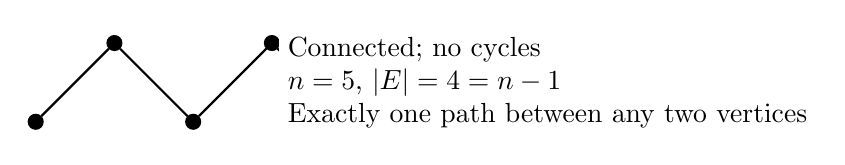
\begin{tikzpicture}[thick,vertex/.style={circle,draw=black,fill=black,inner sep=0pt,minimum size=5pt}]
\node[vertex] (a) at (0,0) {}; \node[vertex] (b) at (1,1) {}; \node[vertex] (c) at (2,0) {}; \node[vertex] (d) at (3,1) {}; \node[vertex] (e) at (4,0) {};
\draw (a)--(b)--(c)--(d)--(e);
\node[draw=none,rectangle,fill=white,align=left] at (6.5,0.5) {Connected; no cycles\\$n=5$, $|E|=4=n-1$\\Exactly one path between any two vertices};
\end{tikzpicture}
\caption{This five-vertex tree displays the equivalent edge-count and unique-path properties.}
\end{figure}
\begin{proof}
(i)$\Rightarrow$(ii): connectedness gives at least one path. If there were two different paths between the same vertices, follow them from their first divergence to their next meeting; together they contain a cycle. This contradicts that $T$ is acyclic.

(ii)$\Rightarrow$(i): a unique path for every pair gives connectedness. A cycle would give two different paths between two of its vertices, so there is no cycle.

For the edge count, use induction on $n$. A tree with at least two vertices has a leaf (an endpoint of a longest path; it cannot have another neighbour without extending the path or creating a cycle). Removing the leaf and its one edge leaves a tree. Induction gives $n-2$ remaining edges, so the original has $n-1$. Conversely, if a connected graph has more than $n-1$ edges, build a spanning tree by starting at one vertex and repeatedly adding an edge to a new vertex; this uses $n-1$ edges, so an extra edge closes a cycle. Hence a connected graph with $n-1$ edges is acyclic. Finally, an acyclic graph on $n$ vertices with $c$ components has $n-c$ edges, by applying the tree count to each component. If it has $n-1$ edges, then $c=1$, so it is connected. This proves all directions.
\end{proof}

\begin{example}[A five-site electricity backbone]
In a simplified model with five sites, any spanning tree uses exactly $5-1=4$ links. The tree connects all sites and contains no cycle, so it provides no alternative route if one of its links fails. This edge-count result says nothing about which four links are cheapest; assigning costs turns the problem into finding a minimum spanning tree, as in the optimisation chapter.
\end{example}

\begin{corollary}
Every tree with at least two vertices has at least two leaves. A forest with $n$ vertices and $k$ components has exactly $n-k$ edges.
\end{corollary}
\begin{proof}
The endpoints of a longest path in a tree are both leaves: an additional neighbour would either extend the path or create a cycle. For a forest, apply the tree edge count to each component and add: if their sizes are $n_1,\ldots,n_k$, the total number of edges is $\sum_{i=1}^k(n_i-1)=n-k$.
\end{proof}

\begin{proposition}
Every connected graph contains a spanning tree.
\end{proposition}
\begin{figure}[htbp]
\centering
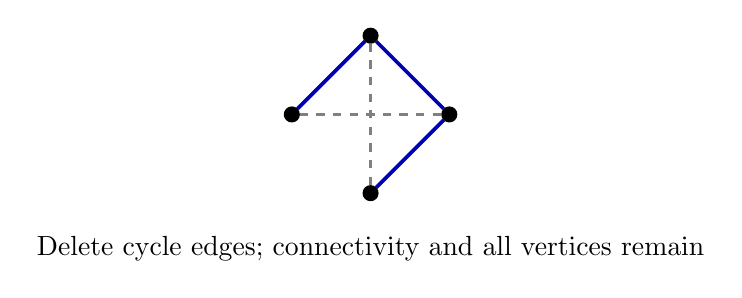
\begin{tikzpicture}[thick,vertex/.style={circle,draw=black,fill=black,inner sep=0pt,minimum size=5pt}]
\node[vertex] (a) at (0,0) {}; \node[vertex] (b) at (1,1) {}; \node[vertex] (c) at (2,0) {}; \node[vertex] (d) at (1,-1) {};
\draw[gray,dashed] (a)--(c) (b)--(d);
\draw[blue!70!black,line width=1.3pt] (a)--(b) (b)--(c) (c)--(d);
\node[draw=none,rectangle,fill=white] at (1,-1.7) {Delete cycle edges; connectivity and all vertices remain};
\end{tikzpicture}
\caption{Repeatedly deleting an edge from a cycle leaves a spanning tree.}
\end{figure}
\begin{proof}
If the graph has a cycle, delete one edge of that cycle; the graph remains connected, because the rest of the cycle still links the edge's endpoints. Repeat until no cycle remains. The resulting connected, acyclic spanning subgraph is a spanning tree.
\end{proof}

Adding one edge to a tree creates exactly one cycle: the new edge joins two vertices already joined by a unique tree path. Removing any edge from a tree disconnects it, since otherwise an alternate route would create a cycle.

\section*{An alkane's bond paths}
In 1875, Arthur Cayley used tree enumeration to count possible alkane structures (structural isomers), rather than to predict the existence of particular molecules.\footnote{A. Cayley, ``On the analytic forms called trees, with applications to the theory of chemical combinations,'' \emph{Report of the 45th Meeting of the British Association for the Advancement of Science} (1875), 257--305.} In a carbon skeleton, vertices represent carbon atoms and edges represent carbon--carbon bonds. Alkane carbon skeletons are trees; a cycle in the carbon skeleton instead indicates a cyclic hydrocarbon.

\begin{figure}[htbp]
\centering
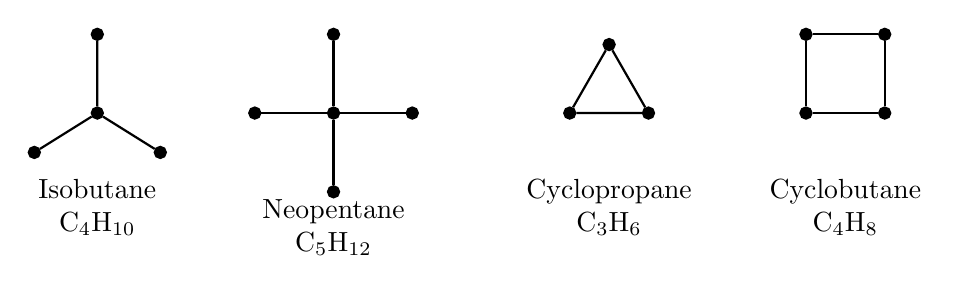
\begin{tikzpicture}[thick,carbon/.style={circle,draw=black,fill=black,inner sep=0pt,minimum size=4pt}]
\begin{scope}
\node[carbon] (i0) at (0,0) {};
\node[carbon] (i1) at (0,1) {};
\node[carbon] (i2) at (-0.8,-0.5) {};
\node[carbon] (i3) at (0.8,-0.5) {};
\draw (i0)--(i1) (i0)--(i2) (i0)--(i3);
\node[draw=none,align=center] at (0,-1.2) {Isobutane\\$\mathrm{C_4H_{10}}$};
\end{scope}
\begin{scope}[shift={(3,0)}]
\node[carbon] (n0) at (0,0) {};
\node[carbon] (n1) at (0,1) {};
\node[carbon] (n2) at (0,-1) {};
\node[carbon] (n3) at (-1,0) {};
\node[carbon] (n4) at (1,0) {};
\draw (n0)--(n1) (n0)--(n2) (n0)--(n3) (n0)--(n4);
\node[draw=none,align=center] at (0,-1.45) {Neopentane\\$\mathrm{C_5H_{12}}$};
\end{scope}
\begin{scope}[shift={(6,0)}]
\node[carbon] (p1) at (0,0) {};
\node[carbon] (p2) at (1,0) {};
\node[carbon] (p3) at (0.5,0.87) {};
\draw (p1)--(p2)--(p3)--(p1);
\node[draw=none,align=center] at (0.5,-1.2) {Cyclopropane\\$\mathrm{C_3H_6}$};
\end{scope}
\begin{scope}[shift={(9,0)}]
\node[carbon] (b1) at (0,0) {};
\node[carbon] (b2) at (1,0) {};
\node[carbon] (b3) at (1,1) {};
\node[carbon] (b4) at (0,1) {};
\draw (b1)--(b2)--(b3)--(b4)--(b1);
\node[draw=none,align=center] at (0.5,-1.2) {Cyclobutane\\$\mathrm{C_4H_8}$};
\end{scope}
\end{tikzpicture}
\caption{Carbon skeletons, with hydrogen atoms omitted. Isobutane and neopentane have tree-shaped carbon skeletons; cyclopropane and cyclobutane contain cycles and are cycloalkanes, not alkanes.}
\end{figure}

\Challenge{} \Uni{} \textbf{Problem.} The \emph{bond graph} of a chemical compound has one vertex per atom and one edge per bond. A hydrocarbon contains only carbon and hydrogen atoms. An alkane of order $n$ has formula $\text{C}_n\text{H}_{2n+2}$, and its bond graph $G$ is a tree in which each carbon vertex has degree 4 and each hydrogen vertex has degree 1. Suppose $E(G)$ is partitioned into $n+1$ edge-disjoint paths, each with two hydrogen endpoints.
\begin{enumerate}
\item Determine the maximum possible number of even-length paths in such a partition. Prove that this maximum can be achieved for every alkane of order $n$, regardless of its structural isomer.
\item Determine all positive integers $n$ for which $E(G)$ can be partitioned into $n+1$ paths that are all even in length.
\end{enumerate}

\begin{figure}[htbp]
\centering
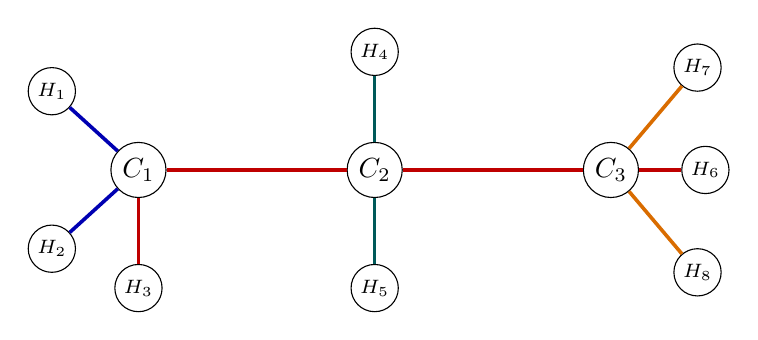
\begin{tikzpicture}[
carbon/.style={circle,draw=black,fill=white,minimum size=7mm,inner sep=1pt,font=\bfseries},
hydrogen/.style={circle,draw=black,fill=white,minimum size=6mm,inner sep=1pt,font=\scriptsize},
pathone/.style={blue!70!black,line width=1.3pt},
pathtwo/.style={red!75!black,line width=1.3pt},
paththree/.style={teal!70!black,line width=1.3pt},
pathfour/.style={orange!85!black,line width=1.3pt}]
\node[carbon] (c1) at (0,0) {$C_1$};
\node[carbon] (c2) at (3,0) {$C_2$};
\node[carbon] (c3) at (6,0) {$C_3$};
\node[hydrogen] (h1) at (-1.1,1) {$H_1$};
\node[hydrogen] (h2) at (-1.1,-1) {$H_2$};
\node[hydrogen] (h3) at (0,-1.5) {$H_3$};
\node[hydrogen] (h4) at (3,1.5) {$H_4$};
\node[hydrogen] (h5) at (3,-1.5) {$H_5$};
\node[hydrogen] (h6) at (7.2,0) {$H_6$};
\node[hydrogen] (h7) at (7.1,1.3) {$H_7$};
\node[hydrogen] (h8) at (7.1,-1.3) {$H_8$};
\draw[pathone] (c1)--(h1) (c1)--(h2);
\draw[pathtwo] (h3)--(c1)--(c2)--(c3)--(h6);
\draw[paththree] (c2)--(h4) (c2)--(h5);
\draw[pathfour] (c3)--(h7) (c3)--(h8);
\end{tikzpicture}
\caption{Propane's bond graph partitioned into four even paths: blue $H_1C_1H_2$ (length 2), red $H_3C_1C_2C_3H_6$ (length 4), teal $H_4C_2H_5$ (length 2), and orange $H_7C_3H_8$ (length 2).}
\end{figure}

\textbf{Solution.} There are $3n+2$ vertices in $G$, so the tree has $3n+1$ edges. The $n+1$ path lengths sum to $3n+1$. If $n$ is even, this sum is odd, so at least one path is odd and at most $n$ paths are even. If $n$ is odd, the edge count is even, giving the upper bound $n+1$. We construct partitions attaining these bounds for every alkane tree.

\textbf{Odd $n$.} Delete the hydrogen leaves to obtain the carbon skeleton $T_C$, a tree on $n$ vertices. Properly two-colour it with classes $X$ and $Y$. Let $H_X$ and $H_Y$ be the hydrogen leaves attached to carbon vertices in $X$ and $Y$, respectively. Since the bond graph is bipartite, the unique path between two hydrogen leaves has even length exactly when both lie in $H_X$ or both lie in $H_Y$.

Label every carbon--hydrogen edge by the colour of its carbon endpoint. For a carbon--carbon edge $uv$, deleting it from $T_C$ gives two subtrees; as $n$ is odd, exactly one has an odd number of vertices. Label $uv$ by the colour of the endpoint in that odd-sized subtree.

At any carbon vertex $w\in X$, deleting $w$ from $T_C$ gives branches $T_1,\ldots,T_k$, where $k=\deg_{T_C}(w)$. The carbon--carbon edge leading to $T_i$ has label $Y$ exactly when $|V(T_i)|$ is odd. Since these branch sizes sum to $n-1$, an even number of them are odd. Thus an even number of the carbon--carbon edges at $w$ have label $Y$. All $4-k$ carbon--hydrogen edges at $w$ have label $X$, so the number of incident edges of each label is even. The same argument with $X$ and $Y$ interchanged applies when $w\in Y$.

At each carbon, pair incident edges with the same label. Following these local pairings partitions all edges into paths: acyclicity rules out closed circuits, and the unpaired endpoints are precisely the hydrogen leaves. Hence there are $(2n+2)/2=n+1$ paths. Along any one path, all edges have the same label; its endpoint leaves therefore both belong to $H_X$ or both to $H_Y$. Each path has even length. This proves the bound $n+1$ for every odd-order alkane tree.

\textbf{Even $n$.} Choose a hydrogen leaf $h_0$ adjacent to a carbon $c_0$. Replace $h_0$ by a new carbon $c_{n+1}$ adjacent to $c_0$ and to three new hydrogen leaves $h_1,h_2,h_3$. The result is an alkane tree $G'$ of odd order $n+1$. Apply the odd-order construction. In its edge labelling, all four edges incident with $c_{n+1}$ have the same label: its carbon--carbon edge is labelled by the colour of $c_{n+1}$, since its side of the carbon skeleton has one vertex, and its three carbon--hydrogen edges receive that colour by definition. We may therefore choose the local pairing there so that $c_{n+1}h_1$ is paired with $c_{n+1}h_2$, and $c_0c_{n+1}$ is paired with $c_{n+1}h_3$.

The resulting even-path partition of $G'$ contains the path $h_1c_{n+1}h_2$ of length 2 and another even path $P$ containing the segment $c_0c_{n+1}h_3$. Delete the first path, and in $P$ replace that two-edge segment by the original edge $c_0h_0$. This shortens $P$ by one, making it odd; the other $n$ paths remain even. These paths partition $E(G)$, so the upper bound of $n$ even paths is attained for every even-order alkane tree.

Consequently,
\[
\max\{\text{number of even paths}\}=
\begin{cases}
n+1,&n\text{ odd},\\
n,&n\text{ even}.
\end{cases}
\]
All $n+1$ paths can be even exactly when $n$ is odd.

\textbf{Structural check.} If $|X|=x$ and $|Y|=y$, then $\sum_{v\in X}\deg_{T_C}(v)=n-1$, so $|H_X|=4x-(n-1)=4x-n+1$; similarly, $|H_Y|=4y-n+1$. Both counts are even exactly when $n$ is odd. The local edge pairings above use the tree structure to turn this parity into an actual path partition.

\section*{A challenge beyond alkane trees}
The previous challenge used the tree structure of alkanes. The next problem allows cycles in the carbon skeleton and combines the handshaking lemma with a double count of triangle--edge incidences.

\Challenge{} \Uni{} \textbf{Problem.} A \emph{saturated hydrocarbon graph} of formula $\mathrm{C}_n\mathrm{H}_m$ ($n,m\geq1$) is a finite simple connected graph $G=(V,E)$ whose vertex set is partitioned into a set $C$ of $n$ carbon vertices and a set $H$ of $m$ hydrogen vertices, such that every $c\in C$ has degree 4 and every $h\in H$ has degree 1. Assume that $H$ is independent (no two vertices of $H$ are adjacent) and that $G$ contains no clique $K_4$. A clique is a set of pairwise adjacent vertices; a clique of size 3 is called a triangle. Let $t$ be the number of triangles in $G$. For an independent set $I\subseteq V$, prove the following and answer the existence question:
\begin{enumerate}
\item Prove that $m$ is even and that
\[
24|I|+2t\leq 12n+21m.
\]
\item Determine all non-negative integers $t$ for which equality can hold for some saturated hydrocarbon graph and some independent set $I$.
\end{enumerate}

\textbf{Solution.} By the handshaking lemma,
\[
4n+m=\sum_{v\in V}\degG(v)=2|E|,
\]
so $m$ is even.

For the inequality, write $I_C=I\cap C$ and $I_H=I\cap H$, and let $E'$ be the set of edges with both endpoints in $V\setminus I$. Since $I$ is independent, every edge outside $E'$ is incident with exactly one vertex of $I$. Therefore
\[
|E|=4|I_C|+|I_H|+|E'|=4|I|-3|I_H|+|E'|,
\]
and hence
\[
4|I|+|E'|=|E|+3|I_H|
\leq \frac{4n+m}{2}+3m
=2n+\frac{7m}{2}.
\]
Multiplying by 6 gives
\[
24|I|+6|E'|\leq 12n+21m. \tag{1}
\]

Let $\mathcal{T}$ be the set of triangles, and count pairs $(e,T)$ with $e\in E'$ an edge of $T$. Each triangle contains at most one vertex of $I$, so it contains at least one edge of $E'$; thus there are at least $t$ such pairs. If an edge $e=xy$ lies in a triangle, then $x,y$ are carbon vertices, since hydrogen vertices have degree 1. The edge $xy$ can belong to at most three triangles, one for each possible common neighbour among the other neighbours of $x$ and $y$. Thus the number of pairs is at most $3|E'|$, and
\[
t\leq 3|E'|,\qquad 2t\leq 6|E'|. \tag{2}
\]
Combining (1) and (2) proves the result. The $K_4$-free condition is not needed for this bound, but it must hold in the examples attaining equality.

For equality, both bounds in the chain must be equalities. In particular, $t=3|E'|$, so $t$ is divisible by 3. Equality in (1) also requires $I_H=H$; equality in the incidence count means each triangle contains exactly one edge of $E'$ and each edge of $E'$ lies in exactly three triangles.

Conversely, let $t=3k$ for a non-negative integer $k$. If $k=0$, take methane: the star $K_{1,4}$ with its centre carbon and four hydrogen leaves, and let $I=H$. Then $n=1$, $m=4$, and equality holds.

For $k\geq1$, take carbon vertices $x_i,y_i$ for $1\leq i\leq k$ and $z_j$ for $1\leq j\leq 2k+1$. Add the edge $x_iy_i$ and join both $x_i$ and $y_i$ to each of $z_{2i-1},z_{2i},z_{2i+1}$. Each $x_i,y_i$ has degree 4. Every interior odd-indexed vertex $z_{2i+1}$ is shared by consecutive pairs and has degree 4; the remaining $k+2$ vertices $z_1,z_{2k+1},z_2,z_4,\ldots,z_{2k}$ have degree 2. To each of these remaining vertices attach two new carbon vertices, each joined to that $z$ and to three new hydrogen leaves. All vertices now have the required degrees. The construction is connected; its only triangles are $\{x_i,y_i,z_{2i-1}\}$, $\{x_i,y_i,z_{2i}\}$, and $\{x_i,y_i,z_{2i+1}\}$ for each $i$, so it is $K_4$-free.

Let $I$ consist of all the $z_j$ and all the hydrogen vertices. These vertices form an independent set, and the only edges with both endpoints outside $I$ are the $k$ edges $x_iy_i$. The graph has
\[
n=2k+(2k+1)+2(k+2)=6k+5,\qquad m=6(k+2)=6k+12,
\]
and $|I|=(2k+1)+m=8k+13$, while it has $t=3k$ triangles. Therefore
\[
24|I|+2t=24(8k+13)+6k=198k+312
=12(6k+5)+21(6k+12)=12n+21m.
\]
Thus equality is possible exactly for the non-negative multiples of 3.

\section*{Exercises}
\begin{enumerate}
\item A tree has 17 vertices. How many edges? If it has 12 edges, how many vertices?
\item Prove that every tree with at least two vertices has at least two leaves.
\item A connected graph has 8 vertices and 10 edges. How many edges must be removed to leave a spanning tree?
\item Explain why a tree with at least two vertices cannot have a universal vertex unless it is a star.
\end{enumerate}
